%==============
%sum

\section{Šum}\label{sec:sum}
Šum je náhodný signál.
Se šumem se často setkáváme v elektronice.
Zde se jedná o nežádaný jev, který zkresluje výsledky.
Setkáváme se s ním také u digitálních fotografii, kde se například projevuje jako změna hodnoty daného pixelu.
V informatice se však šum využívá (například jako zdroj náhodných čísel).
Náhodná čísla (skutečně náhodná čísla) se využívají v kryptografii.
Běžně většinou nemáme k dispozici generátory skutečně náhodných čísel (je k tomu obvykle potřeba specializovaný hardware), proto se používají kongruentní generátory produkující pseudonáhodná čísla.
Seznam hodnot vygenerovaných tímto generátorem je pak považován za šum.
V počítačové grafice se setkáváme s různými druhy generátorů šumu založených na různých druzích generátorů pseudonáhodných čísel.
Na generátory čísel je kladena řada požadavků z pohledu statistiky.
Tyto požadavky je nutné dodržet v případech, kdy hrají důležitou roli (například v simulacích).
V počítačové grafice si však často vystačíme i s jednoduchými implementacemi.
U inter hraje nejdůležitější roli velikost a rychlost.

\subsection{Generátory pseudonáhodných čísel}
Existuje vícero druhů generátorů.
Některé v podobě kongruentního generátoru, jiné v podobě funkce, která má vstupní parametry a vždy pro stejné nastavení parametrů produkuje stejný pseudonáhodný výstup.
Tyto generátory produkují celočíselný výstup s ur\-či\-tým rozsahem.
Je vhodné generátory upravit tak, aby vracely čísla s plovoucí řádovou čárkou v rozsahu $\langle 0,1 \rangle$.
S tímto rozsahem se pak později lépe pracuje.
\begin{itemize}
\item
Kongruentní generátor.
U kongruentního generátoru se vyskytuje inicializační hodnota (takzvané semínko).
Generátor na základě tohoto semínka vygeneruje novou hodnotu a tu do semínka uloží.
Lineární kongruentní generátor má tvar $x_{n+1}=(a \cdot x_n+b) \% m$, kde $a,b,c$ jsou vhodně zvolené konstanty.
Semínko je pak $x_0$.

\item
Generátor založený na funkci.
Tento typ generátoru vrací stejná čísla na základě stejných celočíselných vstupů.
Nalezení takové funkce může být obtížné.
Základem je operace zbytku po celočíselném dělení ($\%$), která se při generování náhodných čísel často používá.
Tvar této funkce, kterou jsem v práci použil je $f(x)=(x^5+x^4+x^3+x^2+x^1) \% N$.
Číslo $N$ je hodnota $2^n,n>0$.
Tento zápis lze pomocí Hornerova schématu zefektivnit: $f(x)=(x(x(x(x(x+1)+1)+1)+1)) \% N $.
Pro vyčíslení jedné hodnoty potřebujeme jen čtyři násobení, čtyři sčítání a jednu operaci modulo.
Experimentálně jsem si ověřil, že pro $N=2^{24}$ funkce vrací pro vstup $x \in \langle 0,N-1 \rangle$ pokaždé jinou hodnotu.
Tento poznatek bychom mohli využít pro konstrukci inverzní funkce.
\end{itemize}

\subsection{Perlinův šum}
\label{subsec:perlin}
Perlinův šum posaný v \cite{KENPERLIN} a v \cite{HUGOPERLIN} je šum založený na šumové funkci.
V počítačové grafice se hojně využívá.
Perlinův šum vrací pro stejné souřadnice stejnou hodnotu v rozsahu $\langle -1,1 \rangle$.
Výsledná hodnota šumu na daných souřadnicích je získána jako součet šumových funkcí o různých frekvencích a amplitudách.
Frekvence se obvykle volí jako násobek základní frekvence $f_0$ mocninou dvě.
Amplituda jednotlivých frekvencí je určena počáteční amplitudou a perzistencí.
Pokud bychom zvolili počáteční amplitudu $A=1$, perzistenci $P=1/2$, tak pro frekvenci $f_0 \cdot 2^n$ je amplituda $a=A \cdot P^n$.
Perlinův šum budeme používat pro generování skyboxů.


\section{Generování šumu půlením intervalu}
Kdybychom vygenerovali sérii hodnot pomocí generátoru náhodných čísel, získali bychom šum, který není pro grafiku příliš vhodný.
Můžeme jej vidět v levé části obrázku \ref{fig:sum}.
Tento šum má hodnoty v sousedních bodech příliš odlišné.
Pro další generování (například textur) je tedy vhodné šum generovat jinak.
Důležité je, aby rozdíly v sousedních bodech byly malé.
Jedním ze způsobů jak to zajistit, je generovat hodnoty s ohledem na již vygenerované hodnoty.
Další vlastností, kterou chceme zaručit je, aby šum na sebe navazoval.
Toto lze zajistit algoritmem půlení intervalu, jehož výsledek je v pravé části obrázku \ref{fig:sum}.
Jak je z tohoto obrázku patrné, šum produkovaný tímto algoritmem je vhodnější pro další generování (například mraků).
\begin{figure}[h]
\centering
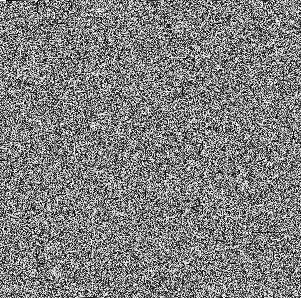
\includegraphics[width=7.5cm,keepaspectratio]{obr/simply_noise.png}
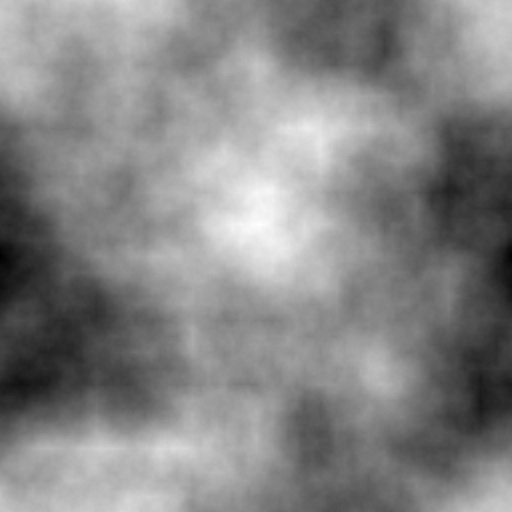
\includegraphics[width=7.5cm,keepaspectratio]{obr/midpoint_noise.jpg}
\caption{Vlevo: šum jako prostá sekvence náhodných čísel. Vpravo: šum vygenerovaný algoritmem půlení intervalu.}
\label{fig:sum}
\end{figure}

Generování šumu pomocí půlení intervalu je dopodrobna popsáno v bakalářské práci \cite{MILET}.
Základem je generátor čísel (v podobě kongruentního generátoru).
Předpokládejme, že chceme vygenerovat jednorozměrný šum reprezentovaný polem o $N$ prvcích s indexy $0,1,\dotsc,N-1$.
Máme k dispozici základní rozsah generátoru $d$ a faktor vyhlazování $m$.
Algoritmus pracuje následovně (jeho vizualizace je v levé části obrázku \ref{fig:midpoint} a výstup v pravé části obrázku \ref{fig:midpoint}):
\begin{enumerate}
\item
Nejprve se vygeneruje náhodná hodnota s rozsahem generátoru $\langle -d,d \rangle$ a uloží se do prvku s indexem $0$.

\item \label{itm:puleni}
Nastaví se nový rozsah $d:=d/m$.

\item
Určí se index $S$ vhodného středu. Je to největší možné číslo $2^n$ takové, že je menší než počet prvků pole ($N$).

\item \label{itm:stred}
Prvek s indexem $S$ má hodnotu součtu váženého průměru a nově vygenerované hodnoty s upraveným rozsahem.
Vážený průměr je počítán z hodnot nejbližších, již vygenerovaných prvků zleva a zprava od $S$, přičemž hodnota váhy je určená vzdáleností jejich indexů od $S$.
Čím je prvek od $S$ vzdálenější, tím má jeho hodnota menší váhu.
Součet vah je roven $1$.
Pokud žádný vygenerovaný prvek zprava neexistuje, použije se prvek s indexem $0$ a vzdálenost je spočítána jako vzdálenost k poslednímu prvku pole plus jedna.
Tímto je zajištěno opakování.

\item
Krokem \ref{itm:stred} nám vznikla dvě pole: jedno s indexy $0,\dotsc,S$ a druhé s indexy $S,\dotsc,N-1$.
Na tato pole se aplikuje tento algoritmus znovu od kroku \ref{itm:puleni}.
Pole však musí mít více než dva prvky.
\end{enumerate}

\begin{figure}[h]
\centering
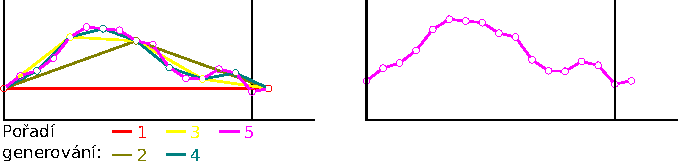
\includegraphics[width=15cm,keepaspectratio]{obr/midpoint.pdf}
\caption{Vlevo: kroky algoritmu půlení intervalu. Vpravo: výsledek algoritmu půlení intervalu.}
\label{fig:midpoint}
\end{figure}

Výše popsaný postup je určen pro jednorozměrný šum.
Více rozměrná varianta je obdobná.
Výpočet hodnoty středního bodu se například pro dvojrozměrný šum nepočítá ze dvou ale ze čtyř okolních bodů.
Podrobně je obecný algoritmu popsán v bakalářské práci \cite{MILET}.
